\documentclass[a4paper,10pt]{article}
\usepackage{Style}
\usepackage{graphicx}
\usepackage{float}
\usepackage{subcaption}


\title{Affinity Research}
\author{Joshua Stoneburner}
\date{August 1st, 2024}
\pagestyle{fancy}
\begin{document}


\maketitle    

\normalsize \textbf{Abstract:}
Opioid addiction remains a public health crisis, showing few signs of letting up, even through the debut of the over the counter drug, Narcan. This study explores the binding affinities of various opioids including carfentanil, BU72, Methadone and Fentanyl against the $\mu$-opioid receptor. This is done using software such as RDKit and AutoDock-Vina to generate conformers and perform docking simulations to build a deeper understanding of receptor-ligand interactions. This analysis focused on three receptor models sourced from mice and humans, showing a vital variation across opioids and receptor structures. These results highlight the necessity for specialized optimization programs and strategies to tackle the unique structure of life. This research greatly contributed to my growing knowledge of this topic and passion for programming. 

\normalsize \textbf{Statement of Originality:}
All of the scripts in my GitHub repository excluding its dependencies are written by me. The concepts I explore in this page are not entirely original as many of them have been deeply researched before. My priority in this research was to focus on learning about the subject matter and to orient where I would like to go from here.

\section{Introduction}
\small
\textbf{Research Context:}

Research pertaining to the biological processes behind opioid addiction has historically been an uphill battle due to the complexity of the involved systems. However, As we have made major advances in computational capabilities - such as machine learning and bioinformatics - there has been a decrease in the gap of knowledge and an increase in available data. This allowed for a leap in our comprehension of these processes, that we otherwise, would have greater difficulty understanding. 
Opioid addiction- and addiction as a whole, still remains as one of many health crises tormenting humanity. The crisis of addiction is a multidisciplinary issue that is in dire need of devoted specialists. 

Between 2019 and 2022 there was an estimated increase in Opioid related overdose deaths of 34,321 people. The drastic increase in overdoses between 2019 and 2022 can partially be attributed to the introduction of synthetic opioids (fentanyl and its variations) to our streets around 2020 and the ongoing mental health crises. The number of opioid involved overdose deaths decreased by only 3,098 people between 2022 and 2023, falling from 84,181 to 81,083 people. Of the 111,029 total overdose deaths reported by the CDC in 2022, opioids make up 75.82 percent. A statistic that went down to 75.4 percent in 2023. This is an incredibly concerning statistic. The marginal drop in opioid deaths between these two years, in spite of 2023 being the introduction of the over the counter drug Narcan, implies the rate of overdose is still rising. 
 I believe there are solutions that have not yet been exhausted - hidden behind the veil of multidisciplinary discoveries and committed research.[1][2]\\
\\

\begin{raggedleft}\textbf{Research Question:}
\end{raggedleft}
How does a chemical cause the chain reaction of overdose, withdrawal (etc.) and how can these properties be modeled and explored.

\textbf{Objective:}
\begin{itemize}
    \item Develop an understanding of the basics behind receptor binding and the biological processes that follow.
    \item  Create a simulation of that basis and compare the affect of different opioids.
\end{itemize}

\subsection{Literature Review}
\small
I began by researching the interaction between gene expression and opioids, a concept I found was well represented by the enzyme cytochrome p450. 
However, I quickly ran into the issue of a majority of related genetics datasets being sequestered by institutions. This was true for most genetic data related to opioids. This is what pushed me towards simulating docking - as it would teach me about the underlying causes of changes in gene expression pertaining to opioids, while still allowing me freedom in research. Following this decision I wrote some short scripts to manipulate medicare data to show me the frequency and distribution of opioid prescriptions, helping lead to my decision to place emphasis on Methadone. After this, much of the literature I reviewed was related to how the $\mu$-opioid receptor works, where the models I used came from, and the properties of the ligands I used in the docking simulations.

\section{Methodology}
\small
\textbf{Research Design:}
I began by creating a Methadone molecule and a program to optimize its structural energy using the software RDKit. 
This optimization program was then revised to produce conformation energy graphs and iterate over each ligand.
I made this Methadone molecule for both understanding and practice, as well as to compare with models of Methadone from drugbank.
I wrote programs to prepare both ligands and receptors for docking simulation by removing additional structures, optimizing and extracting ligands, as well as removing them.
Finally, I ran my main program which docked every ligand against every receptor and graphed their binding affinities. Docking was completed with AutoDock-Vina. File conversion was done using the software obabel. I refrained from using more software for further analysis. Receptor structures came from the RCSB Protein Data Bank

\section{Results}
\small
\subsection{Conformer Generation}

Looking below at figure 1 - the most chaotic dataset I have from energy optimization, it becomes clear that certain energy levels have low odds of generation within the used optimization programs. In this case, rarely occurring conformation energy levels are closer to the lower and upper bound.

\begin{figure}[H]
    \centering
    \begin{subfigure}{0.45\textwidth}
        \centering
        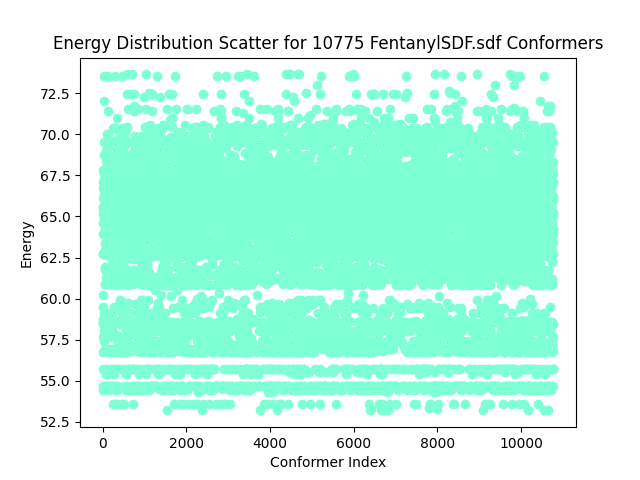
\includegraphics[width=\linewidth]{imgs/FentanylSDF_Energy_Scatter.png}
        \caption{Energy Distribution Scatter Plot}
        \label{fig:image1}
    \end{subfigure}
    \hfill
    \begin{subfigure}{0.45\textwidth}
        \centering
        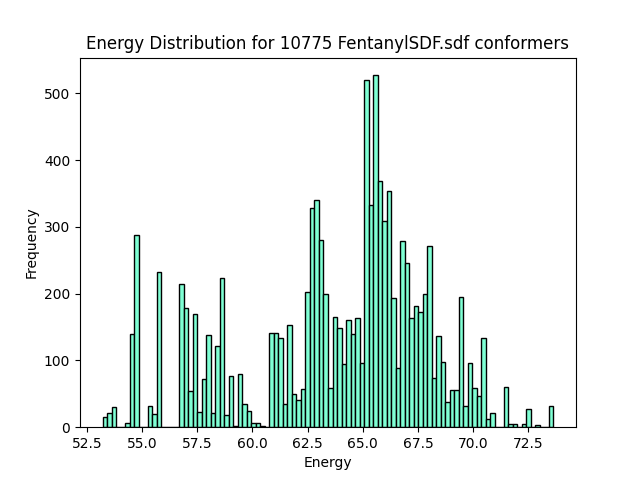
\includegraphics[width=\linewidth]{imgs/FentanylSDF_Energy_Histogram.png}
        \caption{Energy Distribution Histogram}
        \label{fig:image2}
    \end{subfigure}
    \caption{10,775 Fentanyl Conformers}
    \label{fig:comparison}
\end{figure}

The scatter plots included above in figure 2 allow for a better interpretation of the optimization programs abilities. These were both generated from the same run of the optimization program. Meaning that out of two-thousand attempts to generate conformers, the HeroinMOL file could only generate 253. This, as well as both the concentration of conformers between energy levels 70 - 65 and rarity of conformers above 75 in Figure 2: (a) displays the importance of optimization strategy in these programs. I am certain that if I modified the optimization code I could have a higher volume of successfully generated conformers at the cost of the lower bound of energy levels. The requirement of specialized optimization code to handle unique complex molecules, such as heroin, is noteworthy.


\begin{figure}[H]
    \centering
    \begin{subfigure}{0.45\textwidth}
        \centering
        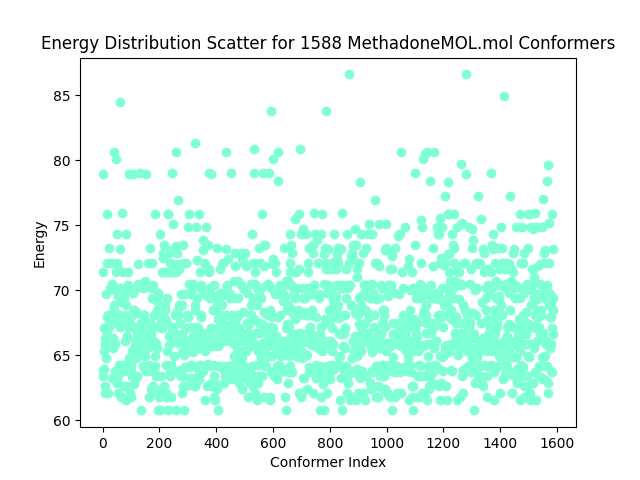
\includegraphics[width=\linewidth]{imgs/MethadoneMOL_Energy_Scatter.png}
        \caption{Methadone Scatter Plot}
        \label{fig:image1}
    \end{subfigure}
    \hfill
    \begin{subfigure}{0.45\textwidth}
        \centering
        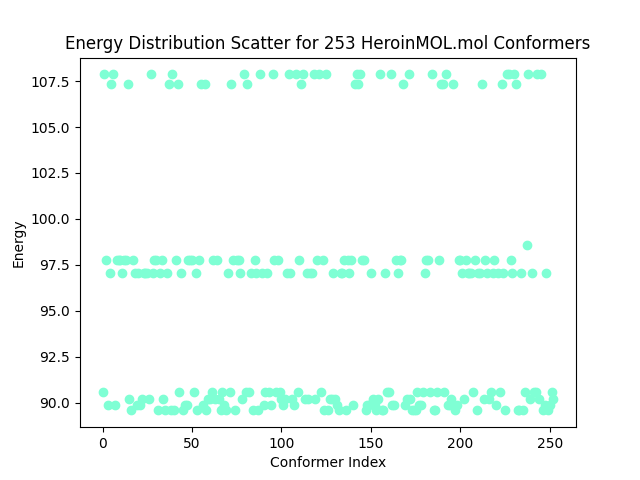
\includegraphics[width=\linewidth]{imgs/HeroinMOL_Energy_Scatter.png}
        \caption{Heroin Scatter Plot}
        \label{fig:image2}
    \end{subfigure}
    \caption{Comparison of MethadoneMOL and HeroinMOL Scatter Plots}
    \label{fig:comparison}
\end{figure}

It should be noted that the energy distribution of the methadone molecule made by me (Figure 3, Page 3) is similar to that of the MethadoneMOL scatter plot in Figure 2: (a). There is a concentration around the 65 range while the low sixties and high seventies onward are rare.

\begin{figure}[H]
    \centering
    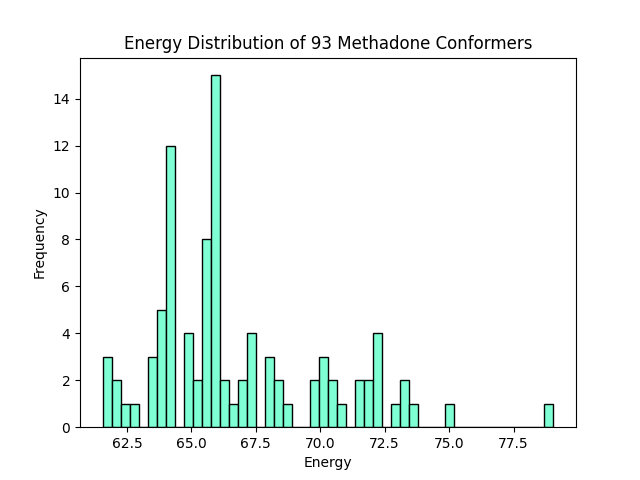
\includegraphics[width=0.5\linewidth]{imgs/Methadone_Energy_Histogram.png}
    \caption{Energy Histogram for My Generated Methadone }
    \label{fig:enter-label}
\end{figure}

\subsection{Docking Simulations}
The following three receptors were used for simulation - the list includes their PDB Id, originally bound ligand, and organism that the models $\mu$-opioid receptor is sourced from, in that order:
\begin{itemize}
    \item 6DDF; DAMGO; Mus Musculus (Mouse)
    \item 8E0G; DU72; Mus Musculus (Mouse)
    \item 8K9K; DAMGO; Homo Sapiens (Human)
\end{itemize}
    DAMGO and DU72 are synthetic opioids.\\
    \\
The binding affinity graphs for the three receptors that I will be comparing are included below in Figure 4 and 5. 
Out of the three, 6DDF was the lowest quality figure, not having any ions or cholesterol molecules to assist in binding, having less accurate simulation coordinates - as well as being from a mouse. When comparing this graphs data with the others, you can see that the range of values was closer, having a narrower gap between the upper and lower bound, as well as every molecule other than fentanyl finding itself binding with a weaker affinity. It should be noted that fentanyl had a binding strength comparable to DU72 in the lower quality model. I believe this is just by chance, as there is nothing obvious that led to this discrepancy. That theory could be tested by rerunning the simulation. There is the possibility that the atoms in the fentanyl model or its overall structure are similar to the originally bound DAMGO molecule leading to the slight increase in binding strength.

The highest quality structure, 8E0G, had the most variety in its binding affinity values - suggesting that this was either due to the originally bound ligand DU72's properties or the inclusion of cholesterol and other third party structures. This structure provided the highest and lowest binding affinities, totaling to a range of 2.04 excluding the outlier of DU72. 

8K9K and 6DDF both have low ranges of 1.06 and 0.75 respectively, after removing the outliers.
It is very possible that the narrowness of binding affinity range in 8K9K and 6DDF can be explained by the receptor previously being bound to DAMGO, although evidence points to this being unlikely since the 8K9K fentanyl binding affinity was notably lower than 8E0G's, which originally housed the opioid DU72 instead.

Other than this the receptor 8K9K is unremarkable as it serves as a middleground between the other two models.



\begin{figure}[H]
    \centering
    \begin{subfigure}{0.45\textwidth}
        \centering
        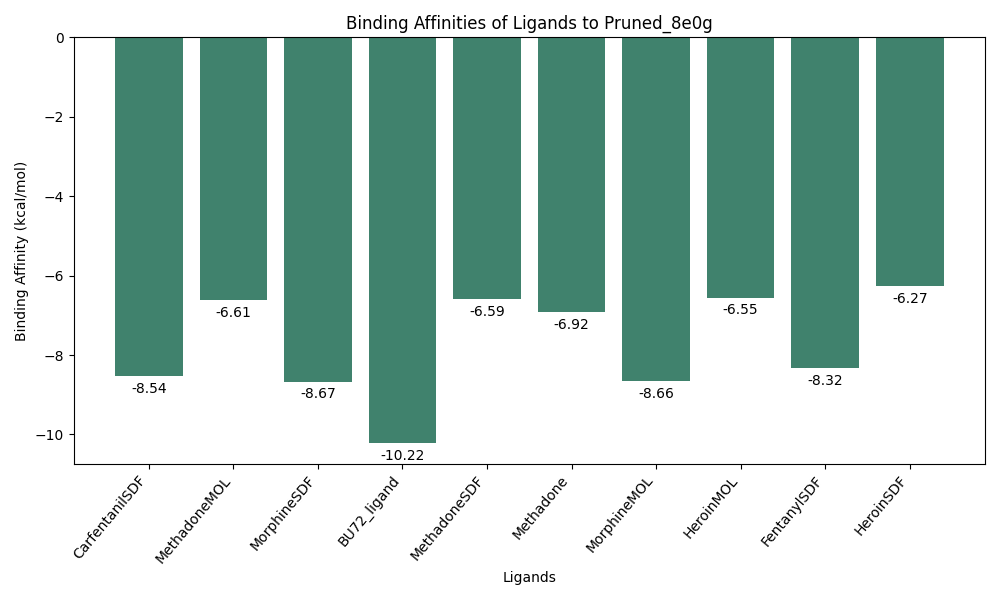
\includegraphics[width=\linewidth]{imgs/Pruned_8e0g_affinities.png}
        \label{fig:image1}
    \end{subfigure}
    \hfill
    \begin{subfigure}{0.45\textwidth}
        \centering
        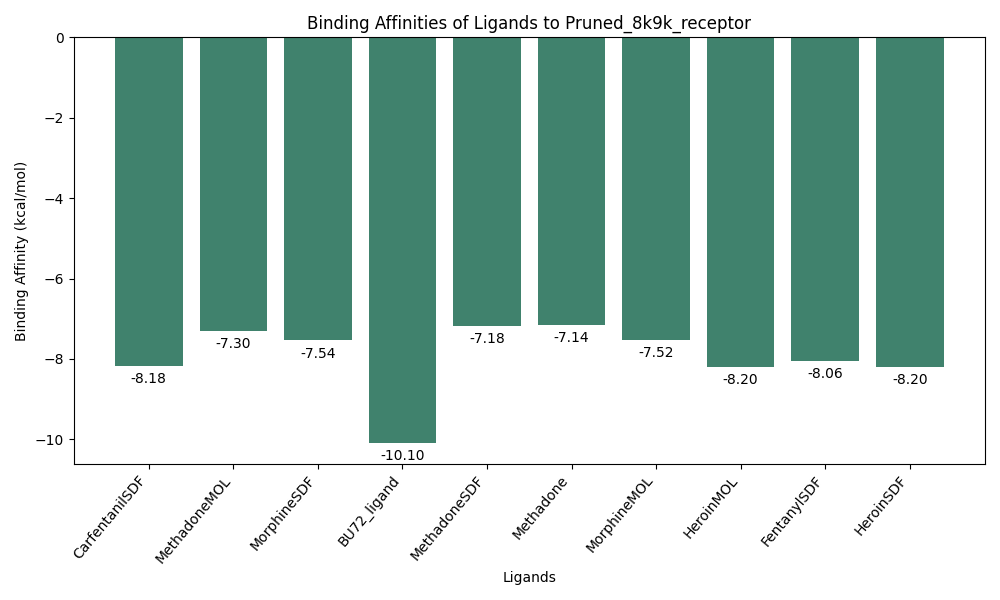
\includegraphics[width=\linewidth]{imgs/Pruned_8k9k_receptor_affinities.png}
        \label{fig:image2}
    \end{subfigure}
    \caption{8E0G and 8K9K Binding Affinity Graphs}
    \label{fig:comparison}
\end{figure}

\begin{figure}[H]
    \centering
    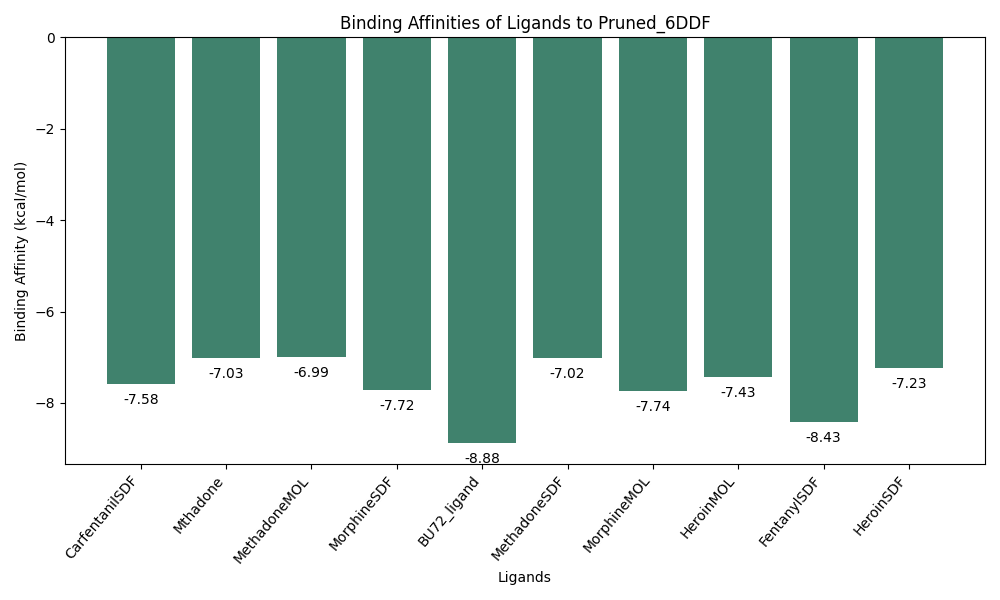
\includegraphics[width=0.5\linewidth]{imgs/Pruned_6DDF_affinities.png}
    \caption{6DDF Binding Affinity Graph}
    \label{fig:enter-label}
\end{figure}

Individual ligand's binding affinities stayed fairly consistent across the .mol and .sdb file type, rarely - if ever, crossing a threshold of 0.30 in their difference. Heroin ligands had an incredibly inconsistent binding affinity, having a range of 1.93 between its highest and lowest value across all receptors. Methadone had consistently the lowest binding affinity other than in 8E0G, while BU72 consistently had the highest. The rest of the molecules had mundane and predictable interactions. \\
\\
My key takeaway from this analysis is that the difference in binding affinity is close to negligible in reality, but leads to a world of difference in an intoxicated individual - and, odds are this is true when it comes to withdrawal. 


\section{Conclusion}
\small
\textbf{Summary of Findings:}

The findings of this research revealed indispensable knowledge about the inner workings of opioid receptors, organic chemistry, computational biology, and biological systems as a whole. These findings further emphasize the importance of accuracy and optimization when gathering data and running simulations. The variation of binding affinities reveals potential hurdles in treating opioid withdrawal - especially in absence of a medical professional. Some examples of hurdles outlined by these results being, dosage of a possible "opioid analgesic", the sensitivity of our body to any form of pharmaceutical, and the difference in every humans brain and bodily structure.\\
\\

\begin{raggedleft}
    \textbf{Limitations:}
    \end{raggedleft}

My study was limited by personal knowledge, data available, computing power, and time. It is possible a majority of these limits will be prevented by the end of my lifetime. In the future I want to do further research on specific segments of the opioid receptor chain reaction, starting from the receptor down. More than this I want to understand where the physical effects of withdrawal come from, and of greater importance, the mental impairment beyond intoxication, that leads to life threatening seizures etc. when going through withdrawal. 
Following my experience at the institute I have developed an inclination to research:
\begin{itemize}
    \item Noradrenaline and its relationship to the psychological effects of withdrawal.
    \item The balance of excitatory and inhibitory neurotransmitter activity.
    \item Biological electric signals i.e. sodium and calcium channels.
    \item Methods of computational biology that find a balance between computational efficiency and accuracy.
    \item Opioids short term disruption and long term damage to the endocrine system.
    \item Opioids long term damage to the endocrine system, desensitization of brain receptors such as dopamine etc. which can be associated with difficulty returning to a "normal" or healthy life. \\
\end{itemize}
\\
Have a wonderful day reader.

\bibliographystyle{plain}
\bibliography{references}
\cite{nida_overdose_2024}
\cite{cdc_health_statistics_2024}

\end{document}



